\section {BISDN} \label{sec:bisdn} %% chapter 3

\begin{figure} [!htbp]
    \centering
    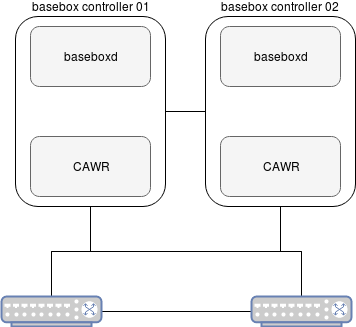
\includegraphics[width=.4\textwidth]{bisdn/basebox}
    \caption{Basebox architecture}
\end{figure}

As the SDN market grows larger and larger in the networking world, new applications and products are developed and improved. Seeing the prevalence of closed source
and proprietary solutions for this market, a need for open products that enable further growth and innovation in cloud DCNs is evident. The main gain in moving from 
vertically integrated solutions, is the decrease of costs involved, as cheaper solutions can be found in whitebox \footnote {whitebox switches are generic switches
that possess no association to a certain vendor} switches and open sourced networking applications. With this motivation, BISDN developed Basebox, a Linux-powered
solution to integrate switches and SDN controllers, allowing for data center  operators to configure and manage networks using linux commands, removing the need for
having to manage several devices with different interfaces and workflows, and adding the capability of running standard networking applications on top of the 
controllers and switches. Basebox also includes the possiblity of running in a failover scenario, by introducing a backup controller for the network, and the
possibility of creating a giant switch abstraction, by adding another controller, Capability AWare Routing (CAWR), and having this manage all the southbound switches.

\subsection {Existing product}

\subsubsection {baseboxd}

\begin{figure} [!htbp]
    \centering
    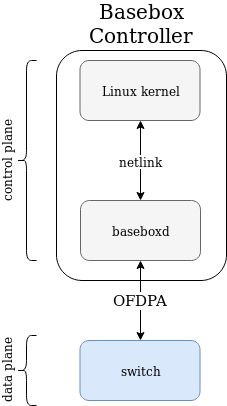
\includegraphics[width=.2\textwidth]{bisdn/baseboxd}
    \caption{Diagram displaying baseboxd's capabilities\cite{bisdn_gmbh_software_2017}}
\end{figure}

baseboxd is a controller daemon connecting whitebox switches with a Linux-based system. The controller communicates with the Linux kernel over netlink 
\footnote{netlink is an Inter-Process Communication's (IPC) socket for exchanging information between the Linux kernel and userspace applications. This interface
provides a communication framework to configure a network's control plane.} and with the switch using the OpenFlow Data Path Abstraction (OF-DPA) which will
represent the state of the switching infrastructure as part of the Linux networking stack.

\par From the perspective of the switch, the baseboxd listens for OFPT\_PORT\_STATUS async messages, and updates the state of the interfaces in the Linux
kernel, creating tap interfaces for each port that is up, and deleting them when they go down. On the controller side, the changes done to the interfaces are also
propagated downwards into the switch, for example the addition of VLANs, or setting route to neighbors, and sends the appropriate flow messages via the OpenFlow 
protocol. Since baseboxd responds directly to the relevant netlink messages, it is one of the intended ways to interface with baseboxd. One may use tools such as
iproute2 and systemd-networkd to configure baseboxd through this interface \cite{bisdn_gmbh_software_2017}.

\subsubsection {CAWR}

CAWR is a secondary OpenFlow controller that creates a giant switch abstraction from a set of whitebox switches. This 
giant switch integrates with baseboxd and allows for easy scaling and management of multiple networking devices. As a secondary controller, it is placed in
between baseboxd and the physical switches, and both its northbound and southbound interfaces are OpenFlow, following the OF-DPA standard.

\par CAWR was designed to handle multi-switch configurations, and the current version supports up to two switches. A host can be connected to each of the switches by
a pair of interfaces that have bond \footnote{Network Interface (NIC) bonding is a process of combining two separate network interfaces into a single 
interface. This technique guarantees performance increase and redundancy.} mode configured, and the layer 2 traffic across the physical network is properly
forwarded. Failover mechanisms to deliver uninterrupted operation are present, in the case of port or switch failure.

\par CAWR adds Link-Aggregation Control Procotol (LACP) (IEEE 802.3ad, IEEE 802.1ax) and Link-layer Discovery Protocol (LLDP) -based (IEEE 802.1ab) topology 
discovery to the Basebox setup. CAWR uses LLDP to detect internal links (connections between the switches) to build an initial topology, and bonds that are
discovered via LACP or have been manually configured are added to the topology as well. LACP is also used to continuously monitor the link status and detect port
connections and disconnections on servers that have LACP enabled \cite{bisdn_gmbh_software_2017}.

\begin{figure} [!htbp]
    \centering
    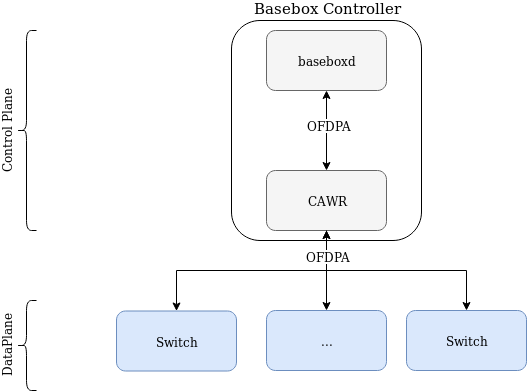
\includegraphics[width=.5\textwidth]{bisdn/cawr}
    \caption{Diagram displaying CAWR's capabilities\cite{bisdn_gmbh_software_2017}}
\end{figure}
